\section{Analysis / Our approach} % (fold)
\label{sec:own_approach}

The \crowdre{} dataset is available in form of a MySQL database dump, but the tables can also be downloaded separated into several \textit{.csv} files\footnote{\url{https://crowdre.github.io/murukannaiah-smarthome-requirements-dataset/}, last visited 2020-01-15}. For our research, we were only interested in the pure requirement sentences (without any ratings, or user characterization added to the data). We could therefore reconstructed the sentences from the \textit{requirements.csv} file only, which is included in the downloaded data.

\colorbox{yellow!30}{ToDo:} Give the approach a name as title!

\subsection{NLP Preprocessing Pipeline} % (fold)
\label{sub:own_pipeline}

\begin{figure}[ht]
  \caption{Our NLP Preprocessing Pipeline and an exemplaric requirement sentence.}
  \centering
    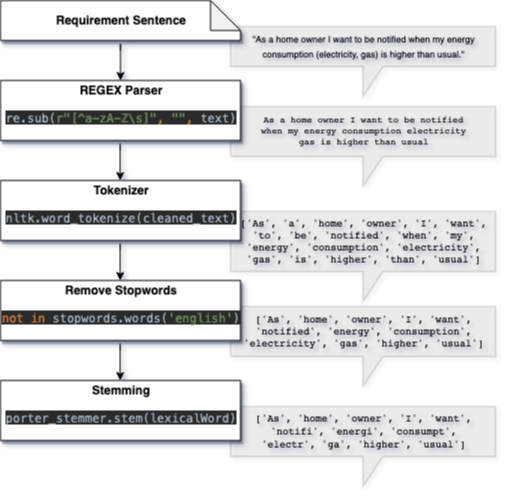
\includegraphics[width=\textwidth]{figures/NLP Pipeline.png}
    \label{fig:nlp_pipeline}
\end{figure}

As initially described in section \ref{sec:nlp} we preprocessed our requirement documents using an NLP pipeline as shown in figure \ref{fig:nlp_pipeline}. Implementing our solution in Python and following the common practice as suggested in \cite{ferrari_natural_2018}, we made use of the NLTK library\footnote{\url{https://www.nltk.org/}, last visited 2020-01-18} to perform the NLP techniques we needed for our analysis. As some of the requirements sentences contained special characters, some initial data cleansing was necessary, to remove these special characters (i.e. spaces, dots, apostrophes, slashes) as they would have otherwise been ranked in the later used bag of words. We used regular expressions as provided by the Python standard library in order to do so. For the tokenization, the stop-word-removal and the stemming we used the functions provided by the NLTK API.
% subsection preprocessing (end)

\subsection{LDA Approach} % (fold)
\label{sub:own_lda}
- how do we process the LDA on our dataset

- Bag of words
- TF/IDF

\subsection{Neural Network} % (fold)
\label{sub:own_neuralnetwork}

\colorbox{yellow!30}{ToDo:} How does our approach with the Neural Network looks like?
